\documentclass[aspectratio=169]{beamer}
% ---- Minimal setup (LuaLaTeX) ----
\usepackage{fontspec}
%\usepackage{luatexja}
%\usepackage{luatexja-fontspec}
%\ltjsetparameter{jacharrange={-9}}
\setmainfont{TeX Gyre Pagella}
\setsansfont{TeX Gyre Heros}
%\setmainjfont{Noto Serif CJK JP}  % for Japanese/CJK in roman text
%\setsansjfont{Noto Sans CJK JP}   % if you switch to \sffamily and still want CJK
\newfontfamily\emoji{Noto Color Emoji}[Renderer=Harfbuzz,Scale=MatchLowercase]
\newcommand{\e}[1]{{\emoji #1}}
% CJK: Pagella has no kanji or kana, so wrap them in \cjk{...} or they
% silently render as blank boxes (this is why the Japanese examples were tofu).
\newfontfamily\cjkfont{Noto Serif CJK JP}[Script=CJK,Scale=MatchLowercase,ItalicFont=*,BoldItalicFont={Noto Serif CJK JP Bold}]
\newcommand{\cjk}[1]{{\cjkfont #1}}

% Dates come from web/weeks.toml via make_dates.py -- never type one.
% Generated by make_dates.py from web/weeks.toml -- do not edit.
% Change the timetable there, then run ./freeze.sh.
% Academic year: 2026

\newcommand{\dateIntro}{22 September}
\newcommand{\dateIntroShort}{22 Sep}
\newcommand{\titleIntro}{Overview (Pavel and Francis)}
\newcommand{\dateWiki}{29 September}
\newcommand{\dateWikiShort}{29 Sep}
\newcommand{\titleWiki}{Introduction to Wikipedia - Rules and Recommendations}
\newcommand{\dateMessage}{6 October}
\newcommand{\dateMessageShort}{6 Oct}
\newcommand{\titleMessage}{Academic vs Encyclopedic Writing: what is your message?}
\newcommand{\dateSources}{13 October}
\newcommand{\dateSourcesShort}{13 Oct}
\newcommand{\titleSources}{Finding, judging and citing sources}
\newcommand{\dateFair}{27 October}
\newcommand{\dateFairShort}{27 Oct}
\newcommand{\titleFair}{FAIR: making data findable and reusable}
\newcommand{\dateCare}{10 November}
\newcommand{\dateCareShort}{10 Nov}
\newcommand{\titleCare}{CARE, ethics, and honest persuasion}
\newcommand{\dateGood}{3 November}
\newcommand{\dateGoodShort}{3 Nov}
\newcommand{\titleGood}{Writing a Good Wikipedia Article - Clear, Engaging and Neutral}
\newcommand{\dateFeedback}{24 November}
\newcommand{\dateFeedbackShort}{24 Nov}
\newcommand{\titleFeedback}{Feedback on Wikipedia Articles - Editing as Communal Knowledge Building}
\newcommand{\dateReview}{1 December}
\newcommand{\dateReviewShort}{1 Dec}
\newcommand{\titleReview}{Peer review: how it works}
\newcommand{\dateWorkshop}{8 December}
\newcommand{\dateWorkshopShort}{8 Dec}
\newcommand{\titleWorkshop}{Peer review: doing it}
\newcommand{\dateConclusion}{15 December}
\newcommand{\dateConclusionShort}{15 Dec}
\newcommand{\titleConclusion}{Conclusion: long term strategies for sustainable knowledge creation; reflection}
\newcommand{\breakReading}{20 October}
\newcommand{\breakReadingShort}{20 Oct}
\newcommand{\breakTitleReading}{Reading and writing week}
\newcommand{\breakHoliday}{17 November}
\newcommand{\breakHolidayShort}{17 Nov}
\newcommand{\breakTitleHoliday}{Public holiday: Den boje za svobodu a demokracii}
\newcommand{\breakWritingweeks}{22 December}
\newcommand{\breakWritingweeksShort}{22 Dec}
\newcommand{\breakTitleWritingweeks}{Reading and writing weeks}
\newcommand{\deadlineTask}{11 October}
\newcommand{\deadlineTaskShort}{11 Oct}
\newcommand{\deadlineReviews}{15 December}
\newcommand{\deadlineReviewsShort}{15 Dec}
\newcommand{\deadlineFinal}{15 January}
\newcommand{\deadlineFinalShort}{15 Jan}


\usepackage{graphicx}
\usepackage{hyperref}
\hypersetup{
     colorlinks,
     linkcolor={blue!50!black},
     citecolor={red!50!black},
     urlcolor={blue!80!black}
   }
% PDF properties shared by the decks and the handouts: \input after hyperref.
% Each document sets its own Title and Author (beamer takes them from \title
% and \author).  Week 5 shows a deck's properties as an example of metadata.
\hypersetup{
     pdfsubject={Open Knowledge for a Sustainable Future: Research, Ethics,
       and Wikipedia (Palacký University Olomouc)},
     pdfkeywords={open knowledge, research ethics, Wikipedia, FAIR data,
       CARE principles, academic writing, peer review},
     pdflang={en},
     pdfinfo={License={CC BY 4.0},
       LicenseURL={https://creativecommons.org/licenses/by/4.0/}}
   }
   % subject, keywords, language, licence
\usepackage{booktabs}
\usepackage{fvextra}   % Verbatim with line breaking (week 5 metadata examples)
\usepackage{microtype}

\newcommand{\txx}[1]{\textbf{\textcolor{blue}{#1}}}

% --- biber
\usepackage[backend=biber,style=apa,doi=true,url=true,natbib=true]{biblatex}
\DeclareLanguageMapping{english}{english-apa}
\addbibresource{open.bib}

% ---- Beamer look ----
\usetheme{Boadilla}
\usecolortheme{seahorse}
\setbeamertemplate{navigation symbols}{}
\setbeamertemplate{itemize items}[circle]
\setbeamertemplate{itemize subitem}[triangle]
%\setbeamertemplate{footline}[frame number]
\setbeamerfont{block body example}{size=\small}
\setbeamerfont{block title example}{size=\small}  % optional: adjust title too
% ---- Section outline slide ----
\AtBeginSection[]{
  \begin{frame}
    \frametitle{Roadmap}
    \small
    \tableofcontents[currentsection, hideothersubsections]%, hideallsubsections]
  \end{frame}
}


% Beamer's quote environment inside an itemize ignores the list indent and
% overflows the right margin by one indent per level.  Boxing it to the
% current line width keeps it inside, wherever it is used.
\let\origquote\quote
\let\endorigquote\endquote
\renewenvironment{quote}%
  {\par\noindent\begin{minipage}{\linewidth}\origquote}%
  {\endorigquote\end{minipage}\par}

% ---- other packages
\usepackage{tikz}

% ---- AI disclosure, shared by every deck so the wording cannot drift ----
% Use inside an itemize: \aicheck
\newcommand{\aicheck}{%
  \item {\small \textbf{Claude Opus 5} \citep{anthropic-claude-opus-5-2026-09-20}
    was used to check the slides: to resolve every
    DOI against Crossref, fetch every URL, and compare each quotation with its
    original.  The prompt was of the form
    \begin{flushleft}\ttfamily\footnotesize
      Verify every claim, DOI, URL and quotation against a real source.  Where
      you cannot verify something, say so rather than guessing --- never
      invent a reference. \\
    \end{flushleft}
    Each correction names the source it was checked against.  Responsibility
    for what remains is mine.}%
}


% ---- Title metadata ----
\title[Peer review]{Open Knowledge for a Sustainable Future:\\ Research, Ethics, and Wikipedia}
\subtitle{Week 7 --- Peer review: how it works}
\author[Bond \& Bednařík]{Francis Bond (\textbf{Academic}) \and Pavel Bednařík (Wiki)}
\institute[UPOL \& Wikimedia]{Palacký University Olomouc \quad | \quad Wikimedia ČR}
\date{}


\begin{document}


% =====================================================================
\begin{frame}
  \titlepage
\end{frame}

\begin{frame}
  \frametitle{Today}
  \small
  \tableofcontents[hideallsubsections]
\end{frame}

% ======================================
% Feedback & Writing: The foundation for peer review
% ======================================

\section{Feedback and Revision}

\begin{frame}{Why feedback?}
\begin{itemize}
  \item First drafts are rarely clear, complete, or well-argued
  \item Feedback (from peers, tutors, self-reflection) helps identify:
    \begin{itemize}
    \item unclear claims
    \item logical gaps
    \item missing evidence
    \item stylistic issues
    \end{itemize}
  \item Better writing is clearer and more persuasive, and when you write about people and their data, more responsible
\end{itemize}
\end{frame}

\begin{frame}{What feedback gives you}
\begin{itemize}
  \item As the writer:
    \begin{itemize}
    \item Another reader's view: it shows your assumptions and blind spots
    \item Fresh eyes on the structure: does the argument build?
    \item A chance to add evidence and answer counter-arguments
    \item A chance to fix style and tone for the audience
    \end{itemize}
  \item As the reader:
    \begin{itemize}
    \item You learn to weigh evidence and spot weak arguments
    \item You see how other people solve the problems you have
    \item Better writing, better discussion
    \end{itemize}
  \item Think of the review you wrote on Moodle: which of these did it do?
\end{itemize}
\end{frame}

\begin{frame}{Feedback as an ethical check}
\begin{itemize}
  \item Writing about people, cultures and data carries responsibility: a reader can catch bad framing, bias or harm you did not see
  \item Facts get checked, sources verified, sensitive topics handled with care
  \item Careful writing builds trust in scholarship as a whole
\end{itemize}
\end{frame}


% =========================
% Week 7 — Peer Review, Trust, and Metrics
% =========================

\section{Peer Review, Trust, and Metrics}

% --- WHAT PEER REVIEW IS
\begin{frame}{What peer review is}
\begin{itemize}
  \item Experts evaluate a manuscript before it is published
  \item Its aims are to:
    \begin{itemize}
      \item Check the \textbf{soundness} of methods and argument
      \item Improve clarity, structure, and contribution
      \item Build \textbf{trust} in published research
    \end{itemize}
  \item Reviewers are gatekeepers and, at best, mentors
\end{itemize}
\end{frame}

% --- TYPES OF PEER REVIEW
\begin{frame}{Types of peer review}
\begin{itemize}
  \item Three models, trading off transparency, fairness and accountability
\end{itemize}

\begin{description}
  \item[Single-blind:] Reviewers know the author's identity, but authors do not know the reviewers
    \begin{itemize}
      \item Common in science and social science
      \item Advantage: reviewers can assess expertise and potential conflicts
      \item Risk: unconscious bias (e.g., by gender, affiliation, language, or region)
    \end{itemize}

  \item[Double-blind:] Neither authors nor reviewers know each other's identity
    \begin{itemize}
      \item Reduces bias (see the WSDM experiment later)
      \item Often used in humanities and linguistics conferences
      \item Risk: less accountability, and reviewers can often guess the authors
    \end{itemize}

  \item[Open review:] Both sides know identities, and sometimes reviews are published
    \begin{itemize}
      \item Transparent, and reviewers get credit for their work
      \item Politer, but reviewers may hold back (see the BMJ trial later)
      \item Used in some open-science and data journals
    \end{itemize}
\end{description}
 \end{frame}



% --- STRENGTHS AND WEAKNESSES
\begin{frame}{Peer review: strengths and weaknesses}
\begin{columns}[T]
\column{0.48\textwidth}
\textbf{Strengths}
\begin{itemize}
  \item Catches errors before publication
  \item Provides expert feedback before publication
  \item A shared standard: ``peer reviewed'' means something
  \item Dialogue within a discipline
\end{itemize}

\column{0.48\textwidth}
\textbf{Weaknesses}
\begin{itemize}
  \item Can be slow, inconsistent, or biased
  \item Overburdens a small reviewer pool
  \item Reviewers rarely check replication
  \item Negative or null results often unpublished (the file-drawer effect)
\end{itemize}
\end{columns}
\end{frame}

% --- REVIEWER 3 (the joke, and the evidence)
\begin{frame}{The third reviewer}
\begin{itemize}
  \item Every academic has a story about the reviewer who sank their paper
    \begin{itemize}
    \item \href{https://www.youtube.com/watch?v=-VRBWLpYCPY}{Scientific Peer
        Review, ca.\ 1945}: a \emph{Downfall} parody --- two good reviews,
      then the third reviewer wants more experiments
    \item \href{https://shitmyreviewerssay.tumblr.com/}{Shit My Reviewers Say}:
      real review comments, collected
    \end{itemize}
  \item The joke has since moved to \textbf{Reviewer 2}
  \item \citet{Peterson2020} tested it on the reviews of one journal
    (\emph{Political Behavior}):
    \begin{itemize}
    \item Reviewer 2 is no more negative than the others
    \item Reviewer 3 is the one most often far below the other reviewers
    \end{itemize}
  \item The point for you: a harsh review is one reader's view ---
    read it for what you can fix
\end{itemize}
\end{frame}

% --- EMERGING ALTERNATIVES (with hyperlinks)
\begin{frame}{Evolving models of peer review}
\begin{itemize}

  \item \textbf{Post-publication review:}
    \begin{itemize}
      \item Articles or datasets are published first, then openly discussed
      \item Examples:
        \href{https://f1000research.com/}{F1000Research},
        \href{https://pubpeer.com/}{PubPeer}
    \end{itemize}

  \item \textbf{Community review:}
    \begin{itemize}
      \item Large-scale collaborative commenting before publication
            (e.g., open preprints, \href{https://github.com/}{GitHub issues}, \href{https://langsci-press.org/openReview/intro}{Open Review at LangSci Press})
      \item Many eyes, in the open
    \end{itemize}

  \item \textbf{Preprint feedback:}
    \begin{itemize}
      \item Early sharing (e.g., \href{https://arxiv.org/}{arXiv},
            \href{https://ling.auf.net/lingbuzz}{LingBuzz}) gets informal feedback before submission
      \item Faster, and it establishes priority (no fear of being scooped)
    \end{itemize}

  \item In all three, review is a conversation that continues after publication
\end{itemize}

\end{frame}


% ================================
% Feedback in Industry: Giving Notes
% ================================
\subsection{Feedback Beyond Academia}

\begin{frame}{Feedback in industry: giving notes}
\begin{itemize}
  \item In film, publishing, games and advertising, feedback is called \txx{notes} \citep{catmull2014creativityinc}
  \item Notes come from editors, producers, managers and clients, usually down a hierarchy
  \item The goal is the same as in academic review:
    \begin{itemize}
      \item make the work better
      \item make sure it does its job for its audience
    \end{itemize}
  \item The constraints differ:
    \begin{itemize}
      \item deadlines, budgets, brand guidelines, lawyers
      \item the writer, the editor and the client may want different things
    \end{itemize}
\end{itemize}

\medskip
\small Video: \href{https://www.youtube.com/watch?v=I1Mr3oKR7oM}{Ed Catmull on the Pixar Braintrust} (Stanford, 8 min) %% SHOW IN CLASS?
\end{frame}

\begin{frame}{How industry notes differ from academic peer review}
\begin{itemize}
  \item \textbf{Hierarchical}: the notes come from someone with authority over the project
  \item \textbf{Goal-driven}: the note serves the project, brand or product
  \item \textbf{Negotiated, up to a point}: creators argue back, but the final call may not be theirs
  \item \textbf{Iterative}: notes, revisions, more notes, approval
  \item \textbf{Success} means the work does what the project needs
\end{itemize}

\end{frame}

\begin{frame}{Best practices from industry feedback culture}
\begin{itemize}
  \item \textbf{Clarity first}: say what the problem is before proposing a fix (the Pixar rule)
  \item \textbf{Respect the creator's intent}: improve the work without imposing your style
  \item \textbf{Prioritise}: not every note can be taken; choose the ones that serve the project
  \item \textbf{Negotiate}: creators can ask what a note means, and push back
  \item \textbf{Shared responsibility}: notes name problems; the creator chooses the fix
\end{itemize}

\end{frame}

\begin{frame}{What students can learn from industry feedback}
\begin{itemize}
  \item You will get feedback from editors, managers, clients and colleagues
  \item What carries over:
    \begin{itemize}
      \item receiving feedback without defensiveness
      \item interpreting conflicting goals
      \item deciding which suggestions to adopt, adapt, or reject
      \item communicating clearly about revisions
    \end{itemize}
\end{itemize}
\end{frame}


% ================================
% Feedback beyond academia
% ================================

\begin{frame}{Feedback cultures beyond academic peer review}
\begin{itemize}
  \item \textbf{Journalism}: editors and fact-checkers check claims against primary sources before publication (academic reviewers rarely check that a citation says what the paper claims)
  \item \textbf{Wikipedia}: articles pass through community review; Good and Featured Article criteria require verifiability and a neutral point of view
  \item \textbf{Code review}: peers review code for bugs, style and maintainability, in public and tied to version control (GitHub pull requests)
  \end{itemize}
\end{frame}


\subsection{Reviewing at the Association for Computational Linguistics}
% ======================================
% ACL CONTEXT & WHY WE STUDY PEER REVIEW
% ======================================

\begin{frame}{Peer review in Computational Linguistics}
\begin{itemize}
  \item Whole communities invest in improving peer review
  \item The Association for Computational Linguistics (ACL) publishes:
    \begin{itemize}
      \item reviewer training guides \citep{acl2023reviewbasics}
      \item best-practice recommendations  \citep{aclarrguidelines}
      \item annual reports analysing what works and what fails \citep{aclcopr2023}
    \end{itemize}
  \item A large conference at scale --- ACL 2025, for example \citep{acl2025pcreport}:
    \begin{itemize}
    \item  8,360 submissions
    \item  1,699 accepted to the main conference (20.3\%), 1,392 as Findings (16.7\%)
      % (/ 1699 8360.0) 0.20322966507177034
      % (/ 1392 8360.0) 0.16650717703349283
    \item  169 Senior Area Chairs, 1,937 Area Chairs, 11,720 reviewers!
    \item Each paper reviewed by three reviewers, the authors respond, the reviewers update their reviews,  the area chairs suggest which papers are accepted, the senior area chairs make the final decisions, \ldots
    \end{itemize}
\end{itemize}
\end{frame}

% ======================================
% BASICS: QUALIFICATION & CONFLICTS
% ======================================

\begin{frame}{Accept reviews only when appropriate (ACL guidelines)}
\begin{itemize}
  \item Before agreeing to review, check:
    \begin{itemize}
      \item \textbf{Expertise}: Can you fairly assess the methods and claims?
      \item \textbf{Conflicts of interest}: shared institution, collaborators, competitors
      \item \textbf{Capacity}: do you have time to read it carefully?
    \end{itemize}
  \item Accepting when you are unqualified or overloaded leads to unfair or rushed reviews
  \item Slightly undermined by the fact that if you submit a paper, someone from the author team must volunteer to review, and owes
        \href{https://aclrollingreview.org/reviewing-workload-adjustment/}{four reviews per submission} (capped at 16 in a cycle), \ldots
      \begin{itemize}
    \item ACL 2025 accepted 20.3\% to the main conference and a further 16.7\% as Findings --- four papers miss the main conference for every one that makes it, and nearly two thirds are turned down altogether
    \item From October 2026 the \href{https://aclrollingreview.org/sustainable-reviewing-2026}{ACL sustainable reviewing policy} goes further:
      \begin{itemize}
      \item each submission needs a qualified service contributor (at most two submissions each)
      \item authors are capped at 20 submissions and 5 first-author submissions a cycle
      \item no registered service, no review: the paper is desk rejected
      \end{itemize}
    \end{itemize}
\end{itemize}

\end{frame}

% ======================================
% STRATEGIC READING
% ======================================

\begin{frame}{Read carefully and generously (ACL guidelines)}
\begin{itemize}
  \item First read: understand the research question and contribution
  \item Second read: evaluate evidence, structure, and clarity
  \item Look for what the author is trying to do
  \item Avoid snap judgments based on style, formatting, or first impressions
\end{itemize}

\end{frame}

% ======================================
% CONSTRUCTIVE, ACTIONABLE FEEDBACK
% ======================================

\begin{frame}{Write constructive, actionable feedback (ACL guidelines)}
\begin{itemize}
  \item Every review should include both:
    \begin{itemize}
      \item \textbf{Strengths}: what works
      \item \textbf{Weaknesses}: what to fix
    \end{itemize}
  \item Make criticisms specific:
    \begin{itemize}
      \item point to a sentence or section
      \item explain why it is unclear
      \item suggest how to fix it
    \end{itemize}
  \item Vague comments (``the paper is confusing'') do not help
\end{itemize}

\end{frame}

% ======================================
% CHECK ETHICS, REPRODUCIBILITY, FAIRNESS
% ======================================

\begin{frame}{Check evidence, ethics, and reproducibility (ACL guidelines)}
\begin{itemize}
  \item A reviewer is responsible for more than novelty
  \item Consider:
    \begin{itemize}
      \item Are claims supported by evidence?
      \item Are methods and data described clearly?
      \item Are ethical implications acknowledged?
      \item Can results be verified or reproduced?
    \end{itemize}
\end{itemize}

\end{frame}

% ======================================
% PROFESSIONALISM & RESPECT
% ======================================

\begin{frame}{Professionalism and respect (ACL guidelines)}
\begin{itemize}
  \item Use a constructive and collegial tone
  \item Avoid dismissive language:
    \begin{itemize}
      \item ``This is trivial''
      \item ``obviously wrong''
      \item ``the authors don't understand''
    \end{itemize}
  \item Remember: reviewers and authors are colleagues
  \item Treat the paper the way you would want yours to be treated
\end{itemize}

\end{frame}

% ======================================
% POWER & RESPONSIBILITY
% ======================================

\begin{frame}{Reviewer power and responsibility (ACL COPR)}
\begin{itemize}
  \item Reviewers gain \textbf{access to unpublished work} before the community
  \item This creates responsibility:
    \begin{itemize}
      \item Never share, quote or use ideas from the manuscript
      \item Never delay a review to gain priority
      \item Never punish papers that challenge your favourite theory
      \item Declare conflicts of interest
    \end{itemize}
  \item \citet{rockwell2005prethics}: a manuscript under review is confidential; do not share it, and do not use its data or ideas in your own work
  \item Peer review runs on trust
\end{itemize}

\end{frame}

% ======================================
% WHAT THIS MEANS FOR STUDENTS
% ======================================

\begin{frame}{What this means for you (student reviewers)}
\begin{itemize}
  \item The same principles apply in the classroom:
    \begin{itemize}
      \item read generously
      \item comment specifically
      \item focus on clarity, evidence, and logic
      \item be respectful and supportive
    \end{itemize}
  \item Practising good peer review improves your own writing:
    \begin{itemize}
      \item you learn what makes an argument work
      \item you see how readers interpret drafts
      \item you build editorial judgment
    \end{itemize}
\end{itemize}
\medskip
\small  Based on ACL reviewer training materials \citep{acl2023reviewbasics, aclarrguidelines, aclcopr2023}.
\end{frame}

% ======================================
% SUMMARY SLIDE
% ======================================

\begin{frame}{ACL-inspired peer review checklist}
\begin{itemize}
  \item Am I qualified and conflict-free?
  \item Have I read the paper carefully (twice)?
  \item Did I identify strengths and weaknesses?
  \item Are my comments specific and actionable?
  \item Did I evaluate ethics, evidence, and reproducibility?
  \item Is my tone respectful and professional?
  \item Have I upheld confidentiality and integrity?
\end{itemize}

\end{frame}



\section{Problems: Bias \& Inequality, (un)Reproducibility}
\subsection{Punktoza}
\begin{frame}{Publish or Perish}

  \begin{itemize}
  \item Academics are under pressure to publish
  \item This is a major part of how they are evaluated
  \item This should lead to more, higher quality publications
  \item But can lead to many more, lower  quality publications
    \begin{itemize}
    \item Or even fraud!
    \end{itemize}
  \item And means we have to review more and more publications
  \end{itemize}

\end{frame}

% --- METRICS: WHY THEY WERE INTRODUCED
\begin{frame}{Metrics: why they were introduced}
\begin{itemize}

  \item Evaluators wanted standard numbers to compare:
    \begin{itemize}
      \item journals (Impact Factor)
      \item researchers (h-index)
      \item institutions (citation counts, productivity)
    \end{itemize}

  \item \textbf{Impact Factor (IF):} citations made in one year to what a journal published in the \emph{two preceding} years, divided by the number of ``citable items'' (research articles and reviews) it published in those two years
  \begin{itemize}
    \item Designed to help libraries choose which journals to buy
    \item A standard criticism is the mismatch between the two halves: the numerator counts citations to \emph{everything} (editorials, letters, news), the denominator counts only the ``citable items''
  \end{itemize}

  \item \textbf{h-index:} a researcher has index $h$ if they have $h$ papers each cited at least $h$ times
  \begin{itemize}
    \item Productivity and influence in one number
  \end{itemize}

  \item Meant to inform expert judgement, not to replace it

\end{itemize}
\end{frame}


% --- METRICS: PROBLEMS, GOODHART, PUNKTOZA
\begin{frame}{Metrics: when measures become targets}
\begin{itemize}

  \item When hiring, promotion, or funding is tied to metrics:
  \begin{itemize}
    \item Researchers optimise for what is counted, not what is meaningful
    \item Citation counts become currency; novelty outranks replication or rigour
  \end{itemize}

  \item \textbf{Goodhart's Law}, as \citet[p.~308]{strathern1997ratings} put it:
  \begin{itemize}
    \item ``When a measure becomes a target, it ceases to be a good measure''
    \item IF and h-index stop measuring anything once people game them
  \end{itemize}

  \item \txx{Punktoza} (``points fever''): publishing to collect evaluation points \citep{kulczycki2017punktoza,kulczycki2017assessing}
  \begin{itemize}
    \item Encourages salami-slicing, low-risk incremental work, quantity over substance
    \item A rational response to points-based national evaluation
  \end{itemize}

\end{itemize}
\vspace*{-1ex}
\end{frame}


\begin{frame}{Goodhart's Law  \href{https://xkcd.com/2899/}{xkcd 2899}}
  \begin{center}
    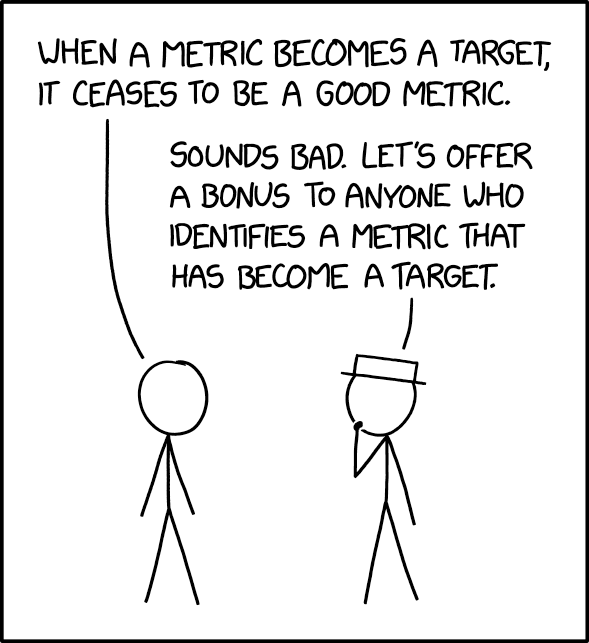
\includegraphics[width=0.40\textwidth]{img/goodharts_law_2x.png}
  \end{center}
\end{frame}

% ===================================
% Bias and Inequality in Peer Review
% ===================================

\subsection{Bias and Inequality in Peer Review}
\begin{frame}{Peer review is not neutral}
\begin{itemize}
  \item Peer review should judge the work alone, but social biases shape outcomes
  \item Studies find bias by gender, prestige and affiliation (next two frames)
  \item The result: the same people stay visible
\end{itemize}
\end{frame}

\begin{frame}{Gender bias and underrepresentation}
\begin{itemize}
  \item A study of 145 journals (1.7 million authors and 740,000 referees) found no penalty for manuscripts by women (if anything, referees and editors treated them slightly more favourably), yet women remain under-represented among reviewers and editors \citep{squazzoni2021genderbias}
  \item An earlier study of 9,000 editors and 43,000 reviewers at one publisher found the same under-representation, and that reviewers tend to be matched with authors like themselves \citep{helmer2017genderbias,murray2018homophily}
  \item In grant-review contexts, women have also been shown to receive lower scores despite similar qualifications
    \citep{wenneras1997nepotism}
  \end{itemize}
\end{frame}

\begin{frame}{Affiliation and prestige bias}
\begin{itemize}
\item Affiliation bias has been measured directly: WSDM 2017 ran a controlled experiment in which every paper got two \emph{single-blind} reviewers and two \emph{double-blind} ones \citep{tomkins2017dblblind}
    \begin{itemize}
    \item The single-blind reviewers were markedly more likely to recommend acceptance for papers by famous authors (odds $\times$1.63) and from top universities ($\times$1.58) or top companies ($\times$2.10)
    \item Their double-blind colleagues, reading the same papers, showed no such advantage --- so double-blinding takes it away
    \end{itemize}
  \item So publication records amplify institutional inequality: the rich get richer
\end{itemize}
\end{frame}

\begin{frame}{Open review --- which is what you just did}
\begin{itemize}
  \item Your reviews went in the Moodle forum: \textbf{signed}, and readable by
    the whole class.  That is \textbf{open review}, and some journals work this
    way (eLife, BMJ, F1000).
  \item \textbf{What blinding buys you}: double-blinding removes the famous-author
    advantage \citep{tomkins2017dblblind}.
  \item \textbf{What signing costs you}: in a randomised trial at the
    \emph{BMJ}, reviewers asked to be identified to the author were
    \textbf{12 points more likely to refuse} to review at all (35\% v 23\%) ---
    but for those who did review, quality, recommendation and time taken were
    \textbf{no different} \citep{vanrooyen1999open}.
\end{itemize}
\vspace{1ex}
\textbf{So, from your own week:}
\begin{itemize}
  \item Did you soften anything because your name was on it?
  \item Did reading other people's reviews change how you wrote yours?
  \item Would you have said more, or less, anonymously?
\end{itemize}
\end{frame}

\begin{frame}{Why these biases happen, and what we can do}
  \begin{itemize}
  \item Why these biases happen
    \begin{itemize}
    \item Reviewers and editors lean on status cues: institution, reputation, familiarity
    \item Reviewing is human work, and unconscious bias (gender, prestige, nationality, career stage) is common
    \item It is structural too: who is asked to review, whose papers get seen, who gets accepted
    \end{itemize}
  \item What this means for us
    \begin{itemize}
    \item As reviewers: judge the content, and notice when you are judging the name
    \item As authors: a rejection is not only about quality
    \item As a community: diverse reviewers and editors, anonymised review where it fits, transparent editorial decisions
    \end{itemize}
  \end{itemize}
\end{frame}


% ===================================
% The Reproducibility Crisis & Why It Matters
% ===================================
\subsection{The Reproducibility Crisis}
\begin{frame}{What is reproducibility / replicability?}
\begin{itemize}
  \item \textbf{Reproducibility:} re-analyse the same data/code to get the same result
  \item \textbf{Replicability:} collect new data under same conditions and test whether the effect holds
  \item Without either, a published finding is provisional \citep{goodman2016reproducibility}
\end{itemize}
\end{frame}

\begin{frame}{The crisis in numbers}
\begin{itemize}
\item In a 2015 project replicating 100 psychology studies, only about 36\% of results were successfully replicated; effect sizes dropped by about 50\% \citep{open2015reproducibility}

  \item A 2016 \textit{Nature} survey of 1,576 researchers, across all the sciences, found over 70\% had tried and failed to reproduce another scientist's results, and 52\% judged that there is a significant crisis \citep{baker2016crisis}
  \item Cancer biology is no better: an eight-year project repeated 50 experiments from 23 high-profile papers, and only 46\% of the replications (51/112) succeeded, with effect sizes a median 85\% smaller \citep{errington2021cancer}
  \item If findings routinely fail to replicate, the literature misleads everyone who builds on it
\end{itemize}

\medskip
\small Video: \href{https://www.youtube.com/watch?v=42QuXLucH3Q}{Veritasium: ``Is Most Published Research Wrong?''} (12 min) %% SHOW IN CLASS?
\end{frame}

\begin{frame}{Causes: why reproducibility fails}
\begin{itemize}
\item Low statistical power (too few subjects): effects that come and go
   \citep{ioannidis2005false}
  \item Publication bias: positive, novel results get published; null results stay in the drawer
  \item Missing code, data and method details: honest researchers make replication impossible by not sharing
  \item Incentives: rewards go to novelty, impact and speed, none to replication
\end{itemize}
\end{frame}

\begin{frame}{FAIR, CARE and good writing help}
\begin{itemize}
  \item FAIR: metadata, shared code and data make re-analysis possible
  \item CARE: honest reporting of context and limitations
  \item Good writing: a reader can tell exactly what was done
  \item Together: more reliable science
\end{itemize}
\end{frame}

% --- CITATION AS TRUST
\begin{frame}{Citation as trust}
\begin{itemize}
  \item A citation says: I read this and trust it enough to build on it
  \item Citations add up to networks of credibility
  \item Not all citations are equal:
    \begin{itemize}
      \item Some endorse, others critique or merely mention
      \item Citation cascades pass on claims no one checked (next slide)
    \end{itemize}
  \item Cite what you have read, and say what you take from it
\end{itemize}
\end{frame}

\begin{frame}{Citogenesis \href{https://xkcd.com/978/}{xkcd 978}}
  \begin{center}
    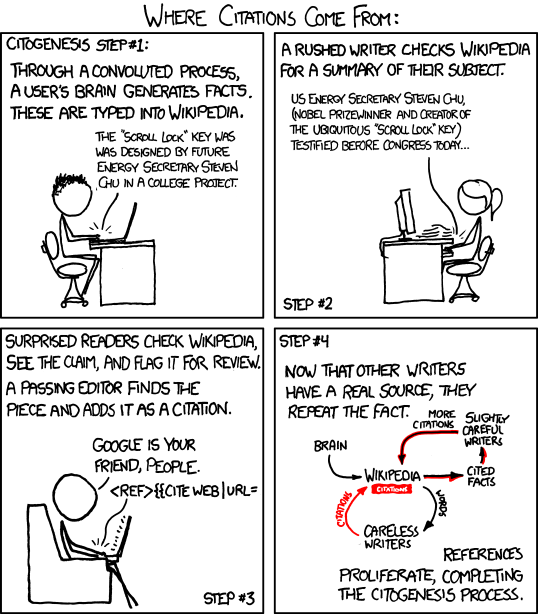
\includegraphics[width=0.4\textwidth]{img/citogenesis.png}
  \end{center}
\end{frame}

% ================================
% AI and Peer Review
% ================================
\subsection{AI and Peer Review}

\begin{frame}{AI in peer review: a known problem}
\begin{itemize}
  \item Large language models (LLMs) are used in academic writing, and in peer review
  \item A 2024 study estimated that 6.5--17\% of peer reviews at major AI conferences may have been substantially written or modified by LLMs \citep{liang2024aireviews}
  \item The tell: \textit{commendable}, \textit{meticulous} and \textit{intricate} rose 10--35 times in frequency
  \item Major publishers all restrict AI in peer review, but not in the same way:
    \begin{itemize}
      \item \textbf{All of them:} never upload the manuscript, or any part of it, to a public AI tool: that alone breaks confidentiality
      \item \textbf{Taylor \& Francis:} AI must not generate the review; it may only improve the language of a review you wrote yourself
      \item \textbf{Sage:} AI may help write and format your review, but not generate it from the manuscript; you remain responsible for its content
      \item \textbf{Springer Nature:} AI may support a reviewer but never replace their judgement; use only secure or institutionally approved tools, and be transparent about it
    \end{itemize}
\end{itemize}
\end{frame}

\begin{frame}{Why AI-generated reviews are problematic}
\begin{itemize}
  \item \textbf{Confidentiality breach}: uploading a manuscript to an LLM shares it with a third party
  \item \textbf{Accountability}: reviewers answer for accuracy and judgement, and an LLM cannot
  \item \textbf{Bias and hallucination}: LLMs repeat biases and produce plausible, wrong critiques
  \item \textbf{Superficiality}: generated reviews are generic and miss the issues an expert would see
  \item \textbf{Trust erosion}: an automated review is no longer an expert's judgement
\end{itemize}
\end{frame}

\begin{frame}{Typical guidance on AI in peer review}
\begin{itemize}
  \item Most journals and conferences now require:
    \begin{itemize}
      \item Disclosure of any AI assistance in writing or reviewing
      \item Human accountability for all submitted content
      \item No uploading of confidential manuscripts to AI tools
    \end{itemize}
  \item Acceptable uses (with disclosure):
    \begin{itemize}
      \item Grammar and spell-checking
      \item Improving clarity of your own writing
    \end{itemize}
  \item Unacceptable uses:
    \begin{itemize}
      \item Generating review text
      \item Summarising or analysing manuscripts you are reviewing
      \item Submitting AI-generated content as your own expert judgment
    \end{itemize}
\end{itemize}
\end{frame}


\begin{frame}{Acknowledgements}

  \begin{itemize}
 \item I have had over 200 papers reviewed (thanks reviewers!)
 \item I have peer reviewed over 2,000 conference papers, 100 journal papers, 10 PhDs, 2 Habilitations, and many grants
  \item \textbf{GPT-4o} in ChatGPT \citep{openai-chatgpt-2025-03-14} was used to format the references, and generate a first draft of the slides
  \aicheck
  \end{itemize}

\end{frame}


% ====================================================
\begin{frame}[allowframebreaks]
\frametitle{References}
\printbibliography[heading=none]
\end{frame}


\end{document}
%%% Local Variables:
%%% coding: utf-8
%%% mode: latex
%%% TeX-engine: luatex
%%% End:
